%%%%%%%%%%%%%%%%%%%%%%%%%%%%%%%%%%%%%%%%%
% Structured General Purpose Assignment
% LaTeX Template
%
% This template has been downloaded from:
% http://www.latextemplates.com
%
% Original author:
% Ted Pavlic (http://www.tedpavlic.com)
%
% Note:
% The \lipsum[#] commands throughout this template generate dummy text
% to fill the template out. These commands should all be removed when 
% writing assignment content.
%
%%%%%%%%%%%%%%%%%%%%%%%%%%%%%%%%%%%%%%%%%

%----------------------------------------------------------------------------------------
%	PACKAGES AND OTHER DOCUMENT CONFIGURATIONS
%----------------------------------------------------------------------------------------

\documentclass{article}

\usepackage{fancyhdr} % Required for custom headers
\usepackage{lastpage} % Required to determine the last page for the footer
\usepackage{extramarks} % Required for headers and footers
\usepackage{graphicx} % Required to insert images
\usepackage{listings} % code listings
\usepackage{cprotect}
\usepackage{xifthen}
\usepackage{tabularx}
\usepackage{multirow}
\usepackage{color}
\usepackage{datetime}
\usepackage[normalem]{ulem}

% Margins
\topmargin=-0.45in
\evensidemargin=0in
\oddsidemargin=0in
\textwidth=6.5in
\textheight=9.0in
\headsep=0.25in 

\linespread{1.1} % Line spacing

% Colors
\definecolor{stringcolor}{rgb}{0.58,0,0.82}
\definecolor{kwordcolor}{rgb}{0,0,1.0}
\definecolor{gray}{rgb}{0.5,0.5,0.5}

% Listings
\lstset{basicstyle=\ttfamily}
\lstset{
    language=C,
    basicstyle=\small\ttfamily,
    keywordstyle=\color{kwordcolor},
    stringstyle=\color{stringcolor},
    frame=single,
    numbers=left,
    stepnumber=1,
    numberstyle=\small\color{gray},
    numbersep=10pt,
    morekeywords={uint64_t, uint32_t, uint16_t, uint8_t,
                  int64_t,  int32_t,  int16_t,  int8_t}
}


% Set up the header and footer
\pagestyle{fancy}
\lhead{\hmwkAuthorName} % Top left header
\chead{\hmwkClass: \hmwkTitle} % Top center header
\rhead{\firstxmark} % Top right header
\lfoot{\lastxmark} % Bottom left footer
\cfoot{} % Bottom center footer
\rfoot{Page\ \thepage\ of\ \pageref{LastPage}} % Bottom right footer
\renewcommand\headrulewidth{0.4pt} % Size of the header rule
\renewcommand\footrulewidth{0.4pt} % Size of the footer rule

\setlength\parindent{0pt} % Removes all indentation from paragraphs

%----------------------------------------------------------------------------------------
%	DOCUMENT STRUCTURE COMMANDS
%	Skip this unless you know what you're doing
%----------------------------------------------------------------------------------------

% Header and footer for when a page split occurs within a problem environment
\newcommand{\enterProblemHeader}[1]{
\nobreak\extramarks{#1}{#1 continued on next page\ldots}\nobreak
\nobreak\extramarks{#1 (continued)}{#1 continued on next page\ldots}\nobreak
}

% Header and footer for when a page split occurs between problem environments
\newcommand{\exitProblemHeader}[1]{
\nobreak\extramarks{#1 (continued)}{#1 continued on next page\ldots}\nobreak
\nobreak\extramarks{#1}{}\nobreak
}

%\setcounter{secnumdepth}{0} % Removes default section numbers
\newcounter{homeworkProblemCounter} % Creates a counter to keep track of the number of problems

\newcommand{\homeworkProblemName}{}
\newenvironment{homeworkProblem}[1][Problem \arabic{homeworkProblemCounter}]{ % Makes a new environment called homeworkProblem which takes 1 argument (custom name) but the default is "Problem #"
\stepcounter{homeworkProblemCounter} % Increase counter for number of problems
\renewcommand{\homeworkProblemName}{#1} % Assign \homeworkProblemName the name of the problem
\section{\homeworkProblemName} % Make a section in the document with the custom problem count
\enterProblemHeader{\homeworkProblemName} % Header and footer within the environment
}{
\exitProblemHeader{\homeworkProblemName} % Header and footer after the environment
}

\newcommand{\problemAnswer}[2][]{ % Defines the problem answer command with the content as the only argument
\noindent\framebox[\columnwidth][c]{
\begin{minipage}{0.98\columnwidth}
#2

\ifthenelse{\isempty{#1}}{}{\textbf{Answer: #1.}}
\end{minipage}
} % Makes the box around the problem answer and puts the content inside, with an optional bolded answer
}

\newcommand{\homeworkSectionName}{}
\newenvironment{homeworkSection}[1]{ % New environment for sections within homework problems, takes 1 argument - the name of the section
\renewcommand{\homeworkSectionName}{#1} % Assign \homeworkSectionName to the name of the section from the environment argument
\subsection{\homeworkSectionName} % Make a subsection with the custom name of the subsection
\enterProblemHeader{\homeworkProblemName\ [\homeworkSectionName]} % Header and footer within the environment
}{
\enterProblemHeader{\homeworkProblemName} % Header and footer after the environment
}
   
%----------------------------------------------------------------------------------------
%	NAME AND CLASS SECTION
%----------------------------------------------------------------------------------------

\newcommand{\hmwkTitle}{Project Report} % Assignment title
\newcommand{\hmwkDueDate}{\formatdate{29}{4}{2016}} % Due date
\newcommand{\hmwkClass}{ECEN\ 4593} % Course/class
\newcommand{\hmwkAuthorName}{Brook Hernandez and Austin Glaser} % Your name
\newcommand{\hmwkAuthorNumber}{101-08-7347 and 810-92-4163} % Student Number

%----------------------------------------------------------------------------------------
%	TITLE PAGE
%----------------------------------------------------------------------------------------

\title{
\vspace{2in}
\textmd{\textbf{\hmwkClass:\ \hmwkTitle}}\\
\normalsize\vspace{0.1in}\small{Due\ on\ \hmwkDueDate}\\
\vspace{3in}
}

\author{
\textbf{\hmwkAuthorName} \\
\hmwkAuthorNumber
}
\date{\today} % Insert date here if you want it to appear below your name

%----------------------------------------------------------------------------------------

\begin{document}

\maketitle

%----------------------------------------------------------------------------------------
%	TABLE OF CONTENTS
%----------------------------------------------------------------------------------------

%\setcounter{tocdepth}{1} % Uncomment this line if you don't want subsections listed in the ToC

\newpage
\tableofcontents
\newpage
\lstlistoflistings
\newpage

%----------------------------------------------------------------------------------------
%	Introduction
%----------------------------------------------------------------------------------------

\section{Introduction}

The goal of the Memory Simulation project was to implement a simulator that can simulate and evaluate a memory system with two levels of cache memory and a main memory. Within the system there is a level-1 (L1) instruction cache and a L1 data cache. There is also a unified level-2 (L2) cache which handles requests from both L1 caches. Misses that occur in the L2 cache are handled by main memory. These caches are write-allocate, write-back caches with an 8-entry victim cache. 

\section{Trend Analysis}

\subsection{Miss Rate and Cache Size Analysis}

Compulsory, capacity, and conflict misses have a big effect on the cache miss rate. A compulsory miss occurs when the first access to a block can not be in the cache. Cumpolsory misses do not depend on size, but capacity misses do. If the cache is too small and cannot hold all of the blocks needed during the execution of the program, then misses occur on blocks that were discarded earlier. If the cache has sufficient space for the data, but the block can not be kept because the set is full, then a conflict miss will occur. 

Reducing cache miss rates depends on the miss type. Conflict and compulsory misses can be reduced in several ways. Larger cache blocks can decrease the compulsory miss rate by taking advantage of spatial locality however, it may also increase the miss penalty by requiring more data to be fetched per miss. In addition, they will almost certainly increase conflict misses since fewer blocks can be stored in the cache. Capacity misses can be reduced by making the cache larger as well. 

Comparing our data for the miss rate and the cache sizes, we can see in figures \ref{fig:L1imissvsl1isize}, \ref{fig:l1vsmiss}, and \ref{fig:l2vsmiss}, that as the cache size increases, the miss rates for the most part decrease. We expected this in most cases because as the cache size increases there is less chance of a conflict miss. It can be seen in figure \ref{fig:l2vsmiss} that there is an exception to our expected results. The miss rate for the bzip2 trace increases slightly as the cache size increases. This could be because...

Brook

\begin{figure}[ht]
    \centering
    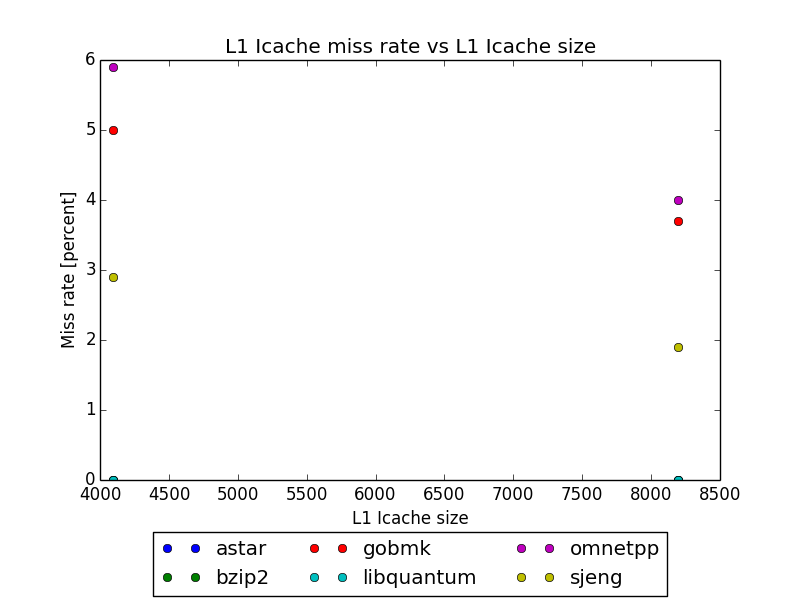
\includegraphics[width=0.75\textwidth]{plots/L1icache_miss_vs_L1icache_size.png}
    \caption{L1 Icache Miss Rate vs L1 Icache Size}
    \label{fig:L1imissvsl1isize}
\end{figure}

\begin{figure}[ht]
    \centering
    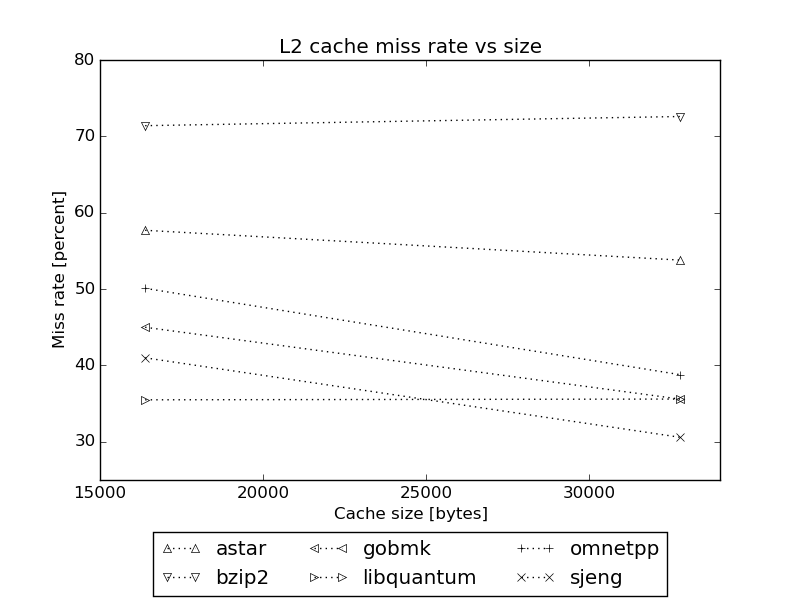
\includegraphics[width=0.75\textwidth]{plots/L2cache_miss_vs_size.png}
    \caption{Size of L2 cache impact on L2 cache miss rate}
    \label{fig:l2vsmiss}
\end{figure}

\begin{figure}[ht]
    \centering
    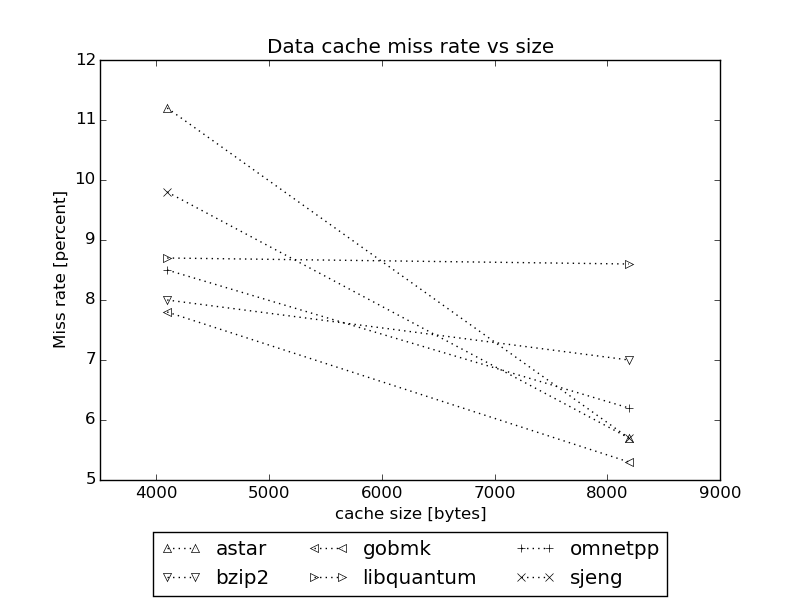
\includegraphics[width=0.75\textwidth]{plots/L1_Dcache_miss_vs_L1_Dcache_size.png}
    \caption{Size of L1 Dcache impact on L1 Dcache miss rate}
    \label{fig:l1vsmiss}
\end{figure}

\subsection{Miss Rate and Cache Associativity Analysis}

Comparing miss rate and cache associativity we can see in figure \ref{fig:L1imissvsl1iassoc}, \ref{fig:l1missvsl1assoc}, and \ref{fig:l2missvsl2assoc} that as the cache associativity increases, the cache miss rate decreases.

Brook

\subsection{CPI and Cache Size Analysis}

Thus far, we've only examined cache miss rates. While this is a reasonable
measure of performance, we've seen in our text that it is not the final story.
For our system, the true measure of performance is the time it takes to execute
a particular trace.

The simplest factor to look at here is the effect of cache size on CPI. Figure
\ref{fig:cpivsl1size} shows the effect of L1 cache size on performance.

It's interesting to see that, while average performance is significantly better
with the larger cache, some traces benefit more than others. This could be due
to several factors. If a trace accesses a large region of memory (a big array,
for instance), or regions mapped to the same block, there will be poor
performance when using a smaller cache, as data is continuously kicked out and
read back in. Conversely, for a trace which spends most of its time in tight
loops, there won't be much advantage to having less memory available.

We also have (again) an anomaly with the bzip2 and astar traces (see listings
\ref{lst:astardefault}, \ref{lst:astarl1small},
\ref{lst:bzip2default}, and \ref{lst:bzip2l1small} for the raw results). CPI is
actually slightly higher with a smaller L1 cache. Intuitively, this doesn't make
much sense. There are cases (identified in the text) where a larger block size
can cause a decrease in performance, but a larger cache should always incur
fewer (or, in the most extreme case, the same number of) misses. It may be
important to note that the traces exhibiting this performance tend to be those
with the best performance even in the default case, showing that they have less
headroom for improvement no matter what memory system they're running on.

\begin{figure}[ht]
    \centering
    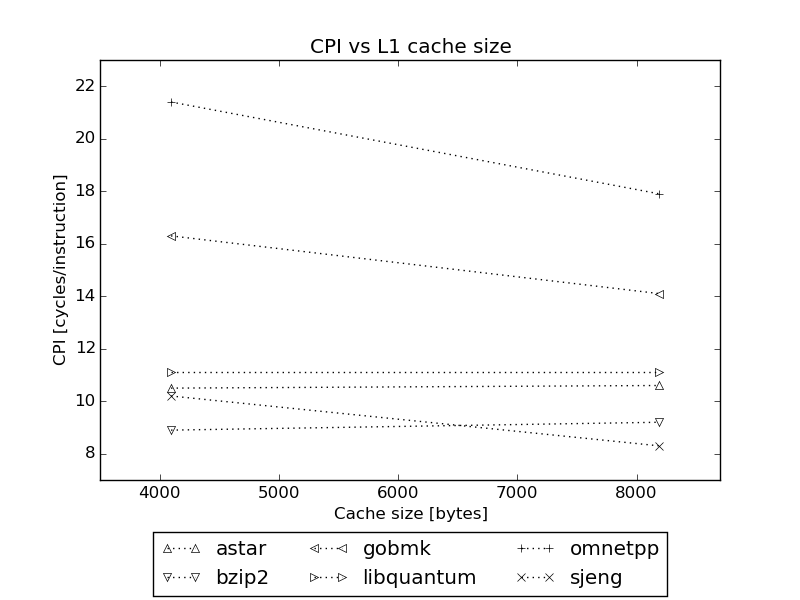
\includegraphics[width=0.75\textwidth]{plots/CPI_vs_L1cache_size.png}
    \caption{CPI vs L1 cache Size}
    \label{fig:cpivsl1size}
\end{figure}

Figure \ref{fig:cpivsl2size} shows the effect of L2 cache size on performance.
The same effect observed above is even more pronounced here, though is primarily
due to the fact that the memory systems with a smaller L2 also have smaller L1
caches (the two being compared are "default" and "All-small").

Interestingly, we see that though bzip2's performance is \emph{nearly} identical
in both cases, both it and astar do exhibit slight improvements in the default
case.

\begin{figure}[ht]
    \centering
    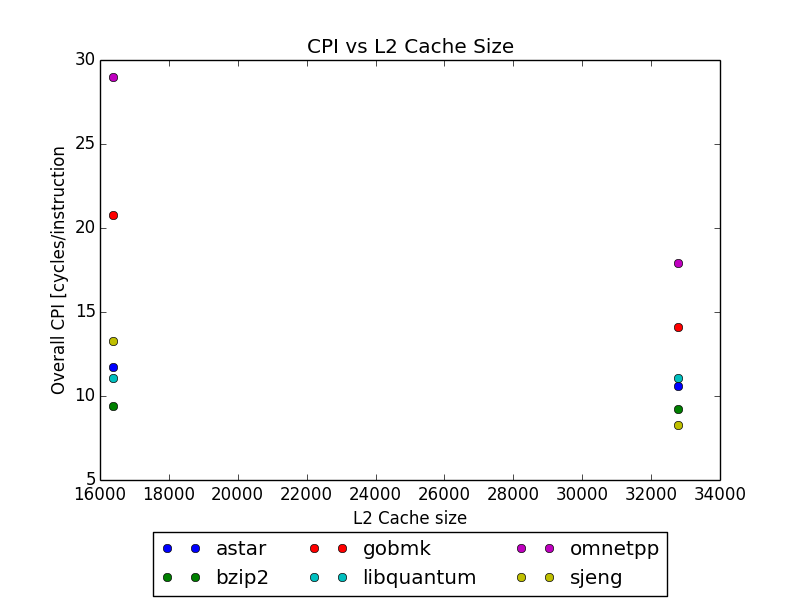
\includegraphics[width=0.75\textwidth]{plots/CPI_vs_L2Cache_size.png}
    \caption{CPI vs L2 Cache size}
    \label{fig:cpivsl2size}
\end{figure}

\subsection{CPI and Cache Associativity Analysis}

We observe, again, that higher associativity has a positive performance impact,
but that that impact is most pronounced with the first few degrees of
associativity. It's also likely that even this effect is slightly blunted, given
that we get some similar effects from implementing a victim cache.

Figures \ref{fig:cpivsl1assoc} and \ref{fig:cpivsl2assoc} show this trend. It's
worth noting that the x-scale for associativity is logarithmic, to better
include the fully-associative case. It's also worth noting that  (for the L1
cache) the fully associative case doesn't fit cleanly into the progression,
since it's the All-FA config, whereas the others only increase L1 associativity.

Since the scale is logarithmic, it's apparent that the increased cost of
implementing very high degrees of associativity is probably not cost effective.
The optimal performance point is likely a 2- or 4-way associative cache.
(although more in-depth analysis of cost-vs-performance will be performed in
section \ref{sec:cost}).

\begin{figure}[ht]
    \centering
    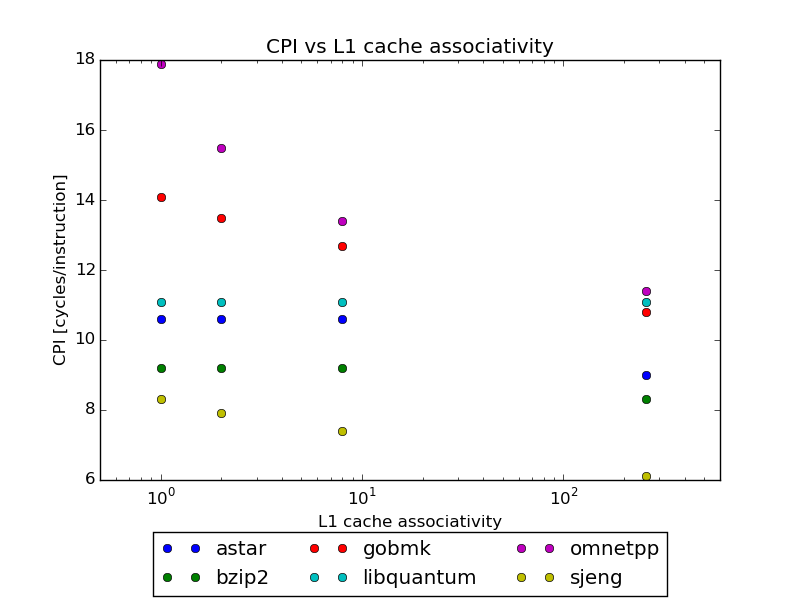
\includegraphics[width=0.75\textwidth]{plots/CPI_vs_L1cache_associativity.png}
    \caption{Performance impact from L1 cache associativity}
    \label{fig:cpivsl1assoc}
\end{figure}

\begin{figure}[ht]
    \centering
    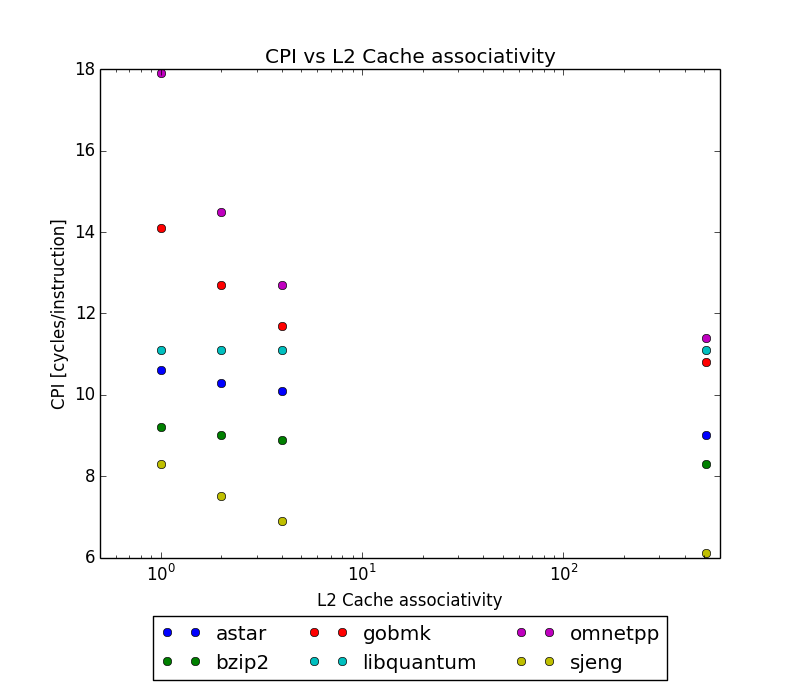
\includegraphics[width=0.75\textwidth]{plots/CPI_vs_L2Cache_associativity.png}
    \caption{Performance impact of L2 cache associativity}
    \label{fig:cpivsl2assoc}
\end{figure}

\subsection{CPI and Costs Analysis} \label{sec:cost}

Figure \ref{fig:cpivstotalcost} includes all memory system configurations,
plotted against their total cost. As might be expected, there's a general trend
to better performance by more expensive systems---but its far from a monotonic
function. This is a good reminder that, if optimizing a memory system, we should
take care to spend money in the right places. Note that this figure only
includes configurations for which we have a full set of results (meaning it
doesn't include results from the sjeng memory bandwidth simulations).

For our hypothetical processor, we'll choose 3 different memory configurations:
a 'bargain basement' variant, where the goal is minimum cost; a
'middle-of-the-road' variant, where the goal is improved performance; and a
'cutting-edge' variant, where the goal is to have maximum performance.

For the bargain-basement processor, we'll evaluate the cheapest three
configurations: All-small, L1-small, and default. Default costs significantly
more than the other two, but provides about the same performance improvement
over L1-small as L1-small does over All-small. For that reason, we would
probably select L1-small as our memory system, since it gives us a significant
improvement over the absolute cheapest option without incurring a huge cost
penalty.

For the middle-of-the-road variant, we'll selecting between the default
configuration, L1-2way, and All-2way. We ignore the L1-small-4way configuration
because it actually performs \emph{worse} than default while costing
\emph{more}. The optimal memory system is probably All-2way, since its again
offers a reasonable performance improvement over its immediate predecessor for a
small cost increase.

Finally, there's only really two possibilities for the cutting-edge variant:
All-4way and All-FA (L1-8way thrown out because, again, it's a loser compared to
All-4way). Realistically, these two configs have fairly similar performance, and
with the exorbitant price tag that three fully-associative caches come with,
it makes sense even for the flagship part to eschew that configuration.
Furthermore, we could explore more 4-way configurations where we increase the
cache sizes or vary the block size and memory bandwidth to achieve optimal
performance.

\begin{figure}[ht]
    \centering
    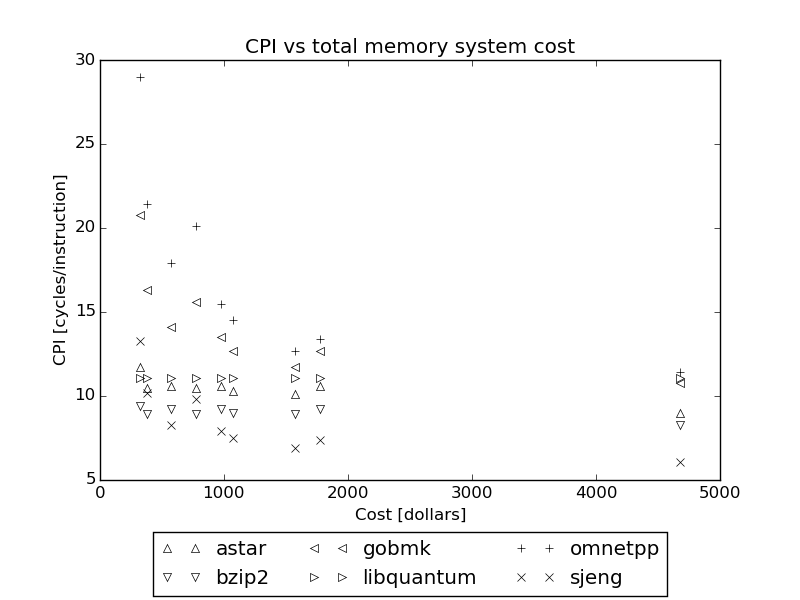
\includegraphics[width=0.75\textwidth]{plots/CPI_vs_Total_memory_system_cost.png}
    \caption{Performance vs Total main memory cost}
    \label{fig:cpivstotalcost}
\end{figure}


\section{Main Memory System Analysis}

One major task in this project was to determine the effect the bandwidth of the
main memory connection has on memory system performance. We only performed the
simulations on the `sjeng` trace, so the plots have less data. Before examining
the results of the simulations, we can make a couple of predictions based around
our knowledge of the memory system's functionality.

The first is that, all other configuration details being equal, there will be no
performance improvement with a bus width greater than 64 bytes. The fastest main
memory access possible will need to transfer a single block of data to or from
the L2 cache, and since that transfer will always be 64 bytes of data, larger
busses will simply be wasted bandwidth.

Secondly, we can expect diminishing returns with each doubling in bandwidth.
There is a constant-time aspect to the memory access (sending the address and
waiting for the memory to be ready), and we're making no changes to that aspect
of the system. As long as this is the case (according to our friend Amdahl),
there is a performance limit which is insurmountable even if we could spend zero
time actually transferring data. Furthermore, these constant time operations
occupy an increasing proportion of our total memory access time.

Now, on to the actual results. Examining figure \ref{fig:cpivsband} shows us
that our predictions are borne out by the actual data -- the largest performance
improvement comes from the first doubling, while later doublings produce
progressively smaller impacts.

We can also look at the relationship between cost and performance (figure
\ref{fig:cpivsmainmemcost}). This is particularly interesting, because the
performance curve flattens out somewhat, becoming somewhat closer to linear.
This means that, from a cost/benefit standpoint, greater memory bandwidths
actually start to look MORE attractive rather than less, even given the
diminishing returns outlined above.

It begins to make sense in light of the chosen cost function, which is actually
logarithmic (ignoring latency, it's $\$75 + \$100 \log_2(B / 8)$, where $B$ is
the memory bandwidth in bytes). To us, this seems slightly unrealistic---our
first instinct is that this function should be linear or worse. However, it does
explain the results, and when taken as a given makes higher-bandwidth main
memory interfaces look slightly more attractive.

\begin{figure}[ht]
    \centering
    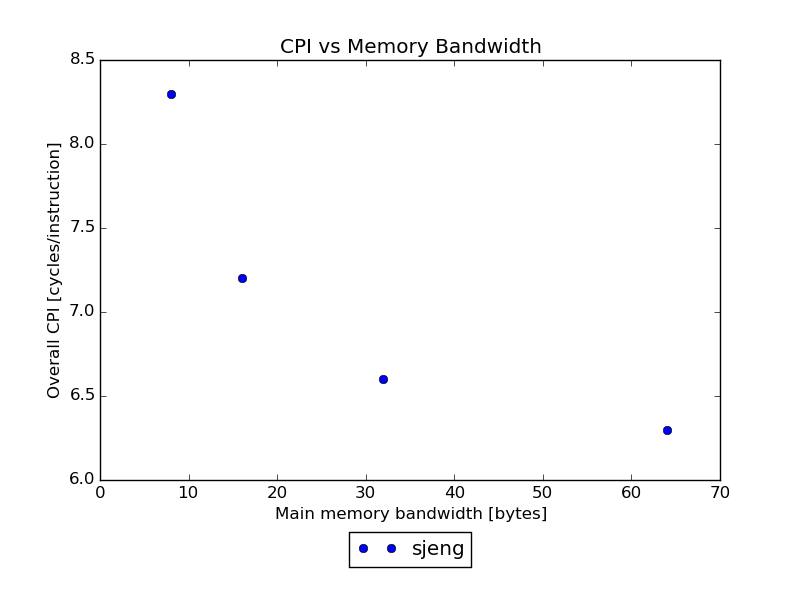
\includegraphics[width=0.75\textwidth]{plots/CPI_vs_Bandwidth.png}
    \caption{Performance impact of main memory bandwidth}
    \label{fig:cpivsband}
\end{figure}

\begin{figure}[ht]
    \centering
    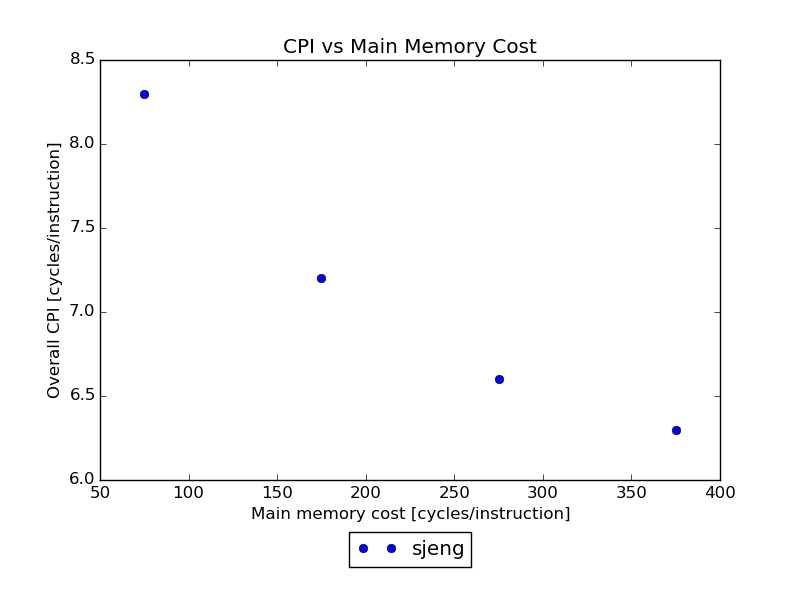
\includegraphics[width=0.75\textwidth]{plots/CPI_vs_Main_Mem_Cost.png}
    \caption{Performance impact of main memory cost}
    \label{fig:cpivsmainmemcost}
\end{figure}

\begin{figure}[ht]
    \centering
    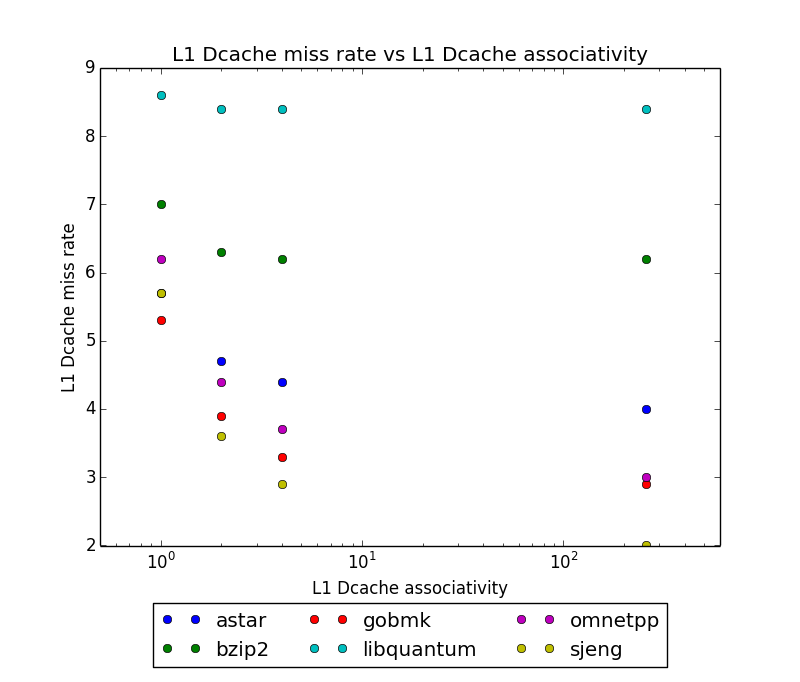
\includegraphics[width=0.75\textwidth]{plots/L1Dcache_miss_vs_associativity.png}
    \caption{L1 Dcache miss rate vs L1 Dcache Associativity}
    \label{fig:l1missvsl1assoc}
\end{figure}

\begin{figure}[ht]
    \centering
    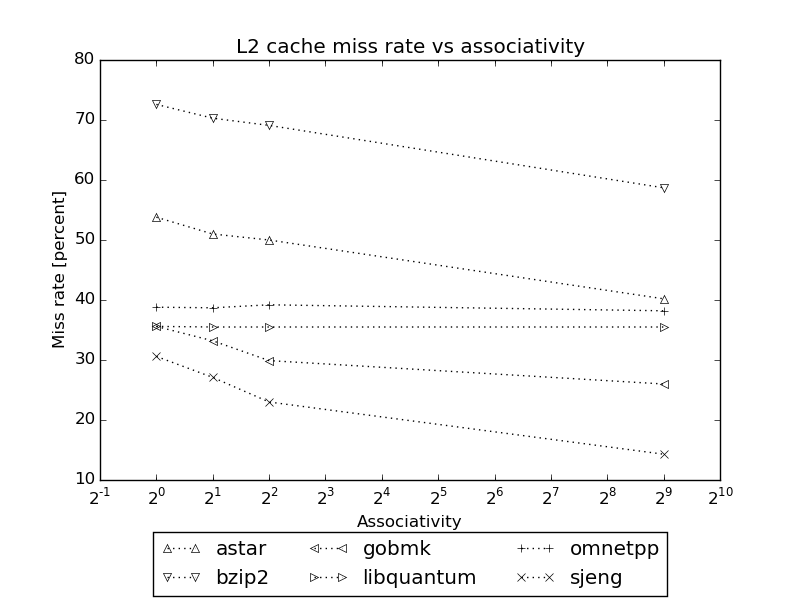
\includegraphics[width=0.75\textwidth]{plots/L2cache_miss_vs_L2cache_associativity.png}
    \caption{L2 cache miss rate vs L2 cache Associativity}
    \label{fig:l2missvsl2assoc}
\end{figure}

\begin{figure}[ht]
    \centering
    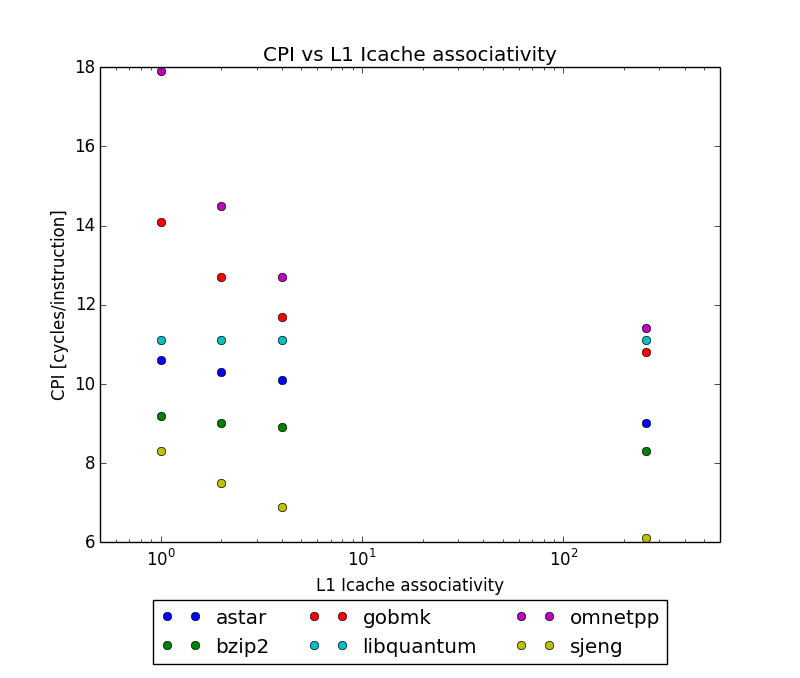
\includegraphics[width=0.75\textwidth]{plots/CPI_vs_L1icache_assoc.png}
    \caption{Performance vs L1 Icache Associativity}
    \label{fig:cpivsl1iassoc}
\end{figure}

\begin{figure}[ht]
    \centering
    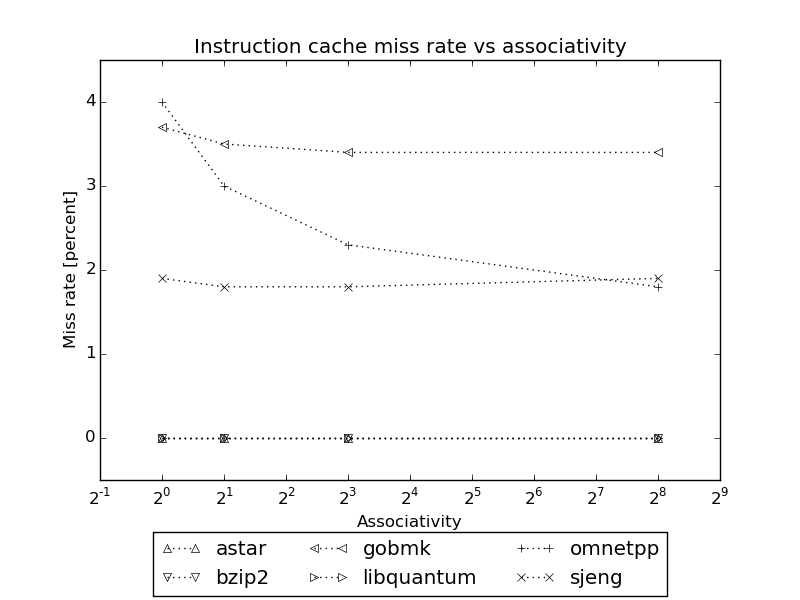
\includegraphics[width=0.75\textwidth]{plots/L1icache_miss_vs_L1icache_Assoc.png}
    \caption{L1 Icache Miss Rate vs L1 Icache Associativity}
    \label{fig:L1imissvsl1iassoc}
\end{figure}


\section{Conclusions}

It's obvious from this report that, as was stated in class, there are simply too
many variables in the design of a cache to perform an exhaustive search of the
configuration space. Instead, a cache designer must use her intuition to guide
the particular paths she explores.

In spite of this, if we had more time to invest in this project, we would
investigate some of the design parameters which were not varied for this
project. Most interestingly would be to verify some of our assumptions about the
performance impact of the victim cache, or different sizes of the same.
It would be especially interesting to compare the performance impact of a victim
cache in the direct-mapped case versus when when a higher-associativity is used.

\clearpage
\appendix
\section{Simulation Results}

This section contains the raw printouts of all simulation results. It's
organized alphabetically by trace, and then alphabetically by configuration
name.

\clearpage
\subsection{Results for astar trace}

\lstinputlisting[caption=astar All-2way Results,
                 firstline=6,
                 lastline=53,
                 language=,
                 label=lst:astarall2way]{../../results/astar.All-2way}
\clearpage

\lstinputlisting[caption=astar All-4way Results,
                 firstline=6,
                 lastline=53,
                 language=,
                 label=lst:astarall4way]{../../results/astar.All-4way}
\clearpage

\lstinputlisting[caption=astar All-FA Results,
                 firstline=6,
                 lastline=53,
                 language=,
                 label=lst:astarallfa]{../../results/astar.All-FA}
\clearpage

\lstinputlisting[caption=astar All-small Results,
                 firstline=6,
                 lastline=53,
                 language=,
                 label=lst:astarallsmall]{../../results/astar.All-small}
\clearpage

\lstinputlisting[caption=astar Default Results,
                 firstline=6,
                 lastline=53,
                 language=,
                 label=lst:astardefault]{../../results/astar.default}
\clearpage

\lstinputlisting[caption=astar L1-2way Results,
                 firstline=6,
                 lastline=53,
                 language=,
                 label=lst:astarl12way]{../../results/astar.L1-2way}
\clearpage

\lstinputlisting[caption=astar L1-8way Results,
                 firstline=6,
                 lastline=53,
                 language=,
                 label=lst:astarl18way]{../../results/astar.L1-8way}
\clearpage

\lstinputlisting[caption=astar L1-small Results,
                 firstline=6,
                 lastline=53,
                 language=,
                 label=lst:astarl1small]{../../results/astar.L1-small}
\clearpage

\lstinputlisting[caption=astar L1-small-4way Results,
                 firstline=6,
                 lastline=53,
                 language=,
                 label=lst:astarl1small4way]{../../results/astar.L1-small-4way}
\clearpage

\subsection{Results for bzip2 trace}

\lstinputlisting[caption=bzip2 All-2way Results,
                 firstline=6,
                 lastline=53,
                 language=,
                 label=lst:bzip2all2way]{../../results/bzip2.All-2way}
\clearpage

\lstinputlisting[caption=bzip2 All-4way Results,
                 firstline=6,
                 lastline=53,
                 language=,
                 label=lst:bzip2all4way]{../../results/bzip2.All-4way}
\clearpage

\lstinputlisting[caption=bzip2 All-FA Results,
                 firstline=6,
                 lastline=53,
                 language=,
                 label=lst:bzip2allfa]{../../results/bzip2.All-FA}
\clearpage

\lstinputlisting[caption=bzip2 All-small Results,
                 firstline=6,
                 lastline=53,
                 language=,
                 label=lst:bzip2allsmall]{../../results/bzip2.All-small}
\clearpage

\lstinputlisting[caption=bzip2 Default Results,
                 firstline=6,
                 lastline=53,
                 language=,
                 label=lst:bzip2default]{../../results/bzip2.default}
\clearpage

\lstinputlisting[caption=bzip2 L1-2way Results,
                 firstline=6,
                 lastline=53,
                 language=,
                 label=lst:bzip2l12way]{../../results/bzip2.L1-2way}
\clearpage

\lstinputlisting[caption=bzip2 L1-8way Results,
                 firstline=6,
                 lastline=53,
                 language=,
                 label=lst:bzip2l18way]{../../results/bzip2.L1-8way}
\clearpage

\lstinputlisting[caption=bzip2 L1-small Results,
                 firstline=6,
                 lastline=53,
                 language=,
                 label=lst:bzip2l1small]{../../results/bzip2.L1-small}
\clearpage

\lstinputlisting[caption=bzip2 L1-small-4way Results,
                 firstline=6,
                 lastline=53,
                 language=,
                 label=lst:bzip2l1small4way]{../../results/bzip2.L1-small-4way}
\clearpage

\subsection{Results for gobmk trace}

\lstinputlisting[caption=gobmk All-2way Results,
                 firstline=6,
                 lastline=53,
                 language=,
                 label=lst:gobmkall2way]{../../results/gobmk.All-2way}
\clearpage

\lstinputlisting[caption=gobmk All-4way Results,
                 firstline=6,
                 lastline=53,
                 language=,
                 label=lst:gobmkall4way]{../../results/gobmk.All-4way}
\clearpage

\lstinputlisting[caption=gobmk All-FA Results,
                 firstline=6,
                 lastline=53,
                 language=,
                 label=lst:gobmkallfa]{../../results/gobmk.All-FA}
\clearpage

\lstinputlisting[caption=gobmk All-small Results,
                 firstline=6,
                 lastline=53,
                 language=,
                 label=lst:gobmkallsmall]{../../results/gobmk.All-small}
\clearpage

\lstinputlisting[caption=gobmk Default Results,
                 firstline=6,
                 lastline=53,
                 language=,
                 label=lst:gobmkdefault]{../../results/gobmk.default}
\clearpage

\lstinputlisting[caption=gobmk L1-2way Results,
                 firstline=6,
                 lastline=53,
                 language=,
                 label=lst:gobmkl12way]{../../results/gobmk.L1-2way}
\clearpage

\lstinputlisting[caption=gobmk L1-8way Results,
                 firstline=6,
                 lastline=53,
                 language=,
                 label=lst:gobmkl18way]{../../results/gobmk.L1-8way}
\clearpage

\lstinputlisting[caption=gobmk L1-small Results,
                 firstline=6,
                 lastline=53,
                 language=,
                 label=lst:gobmkl1small]{../../results/gobmk.L1-small}
\clearpage

\lstinputlisting[caption=gobmk L1-small-4way Results,
                 firstline=6,
                 lastline=53,
                 language=,
                 label=lst:gobmkl1small4way]{../../results/gobmk.L1-small-4way}
\clearpage

\subsection{Results for libquantum trace}

\lstinputlisting[caption=libquantum All-2way Results,
                 firstline=6,
                 lastline=53,
                 language=,
                 label=lst:libquantumall2way]{../../results/libquantum.All-2way}
\clearpage

\lstinputlisting[caption=libquantum All-4way Results,
                 firstline=6,
                 lastline=53,
                 language=,
                 label=lst:libquantumall4way]{../../results/libquantum.All-4way}
\clearpage

\lstinputlisting[caption=libquantum All-FA Results,
                 firstline=6,
                 lastline=53,
                 language=,
                 label=lst:libquantumallfa]{../../results/libquantum.All-FA}
\clearpage

\lstinputlisting[caption=libquantum All-small Results,
                 firstline=6,
                 lastline=53,
                 language=,
                 label=lst:libquantumallsmall]{../../results/libquantum.All-small}
\clearpage

\lstinputlisting[caption=libquantum Default Results,
                 firstline=6,
                 lastline=53,
                 language=,
                 label=lst:libquantumdefault]{../../results/libquantum.default}
\clearpage

\lstinputlisting[caption=libquantum L1-2way Results,
                 firstline=6,
                 lastline=53,
                 language=,
                 label=lst:libquantuml12way]{../../results/libquantum.L1-2way}
\clearpage

\lstinputlisting[caption=libquantum L1-8way Results,
                 firstline=6,
                 lastline=53,
                 language=,
                 label=lst:libquantuml18way]{../../results/libquantum.L1-8way}
\clearpage

\lstinputlisting[caption=libquantum L1-small Results,
                 firstline=6,
                 lastline=53,
                 language=,
                 label=lst:libquantuml1small]{../../results/libquantum.L1-small}
\clearpage

\lstinputlisting[caption=libquantum L1-small-4way Results,
                 firstline=6,
                 lastline=53,
                 language=,
                 label=lst:libquantuml1small4way]{../../results/libquantum.L1-small-4way}
\clearpage

\subsection{Results for omnetpp trace}

\lstinputlisting[caption=omnetpp All-2way Results,
                 firstline=6,
                 lastline=53,
                 language=,
                 label=lst:omnetppall2way]{../../results/omnetpp.All-2way}
\clearpage

\lstinputlisting[caption=omnetpp All-4way Results,
                 firstline=6,
                 lastline=53,
                 language=,
                 label=lst:omnetppall4way]{../../results/omnetpp.All-4way}
\clearpage

\lstinputlisting[caption=omnetpp All-FA Results,
                 firstline=6,
                 lastline=53,
                 language=,
                 label=lst:omnetppallfa]{../../results/omnetpp.All-FA}
\clearpage

\lstinputlisting[caption=omnetpp All-small Results,
                 firstline=6,
                 lastline=53,
                 language=,
                 label=lst:omnetppallsmall]{../../results/omnetpp.All-small}
\clearpage

\lstinputlisting[caption=omnetpp Default Results,
                 firstline=6,
                 lastline=53,
                 language=,
                 label=lst:omnetppdefault]{../../results/omnetpp.default}
\clearpage

\lstinputlisting[caption=omnetpp L1-2way Results,
                 firstline=6,
                 lastline=53,
                 language=,
                 label=lst:omnetppl12way]{../../results/omnetpp.L1-2way}
\clearpage

\lstinputlisting[caption=omnetpp L1-8way Results,
                 firstline=6,
                 lastline=53,
                 language=,
                 label=lst:omnetppl18way]{../../results/omnetpp.L1-8way}
\clearpage

\lstinputlisting[caption=omnetpp L1-small Results,
                 firstline=6,
                 lastline=53,
                 language=,
                 label=lst:omnetppl1small]{../../results/omnetpp.L1-small}
\clearpage

\lstinputlisting[caption=omnetpp L1-small-4way Results,
                 firstline=6,
                 lastline=53,
                 language=,
                 label=lst:omnetppl1small4way]{../../results/omnetpp.L1-small-4way}
\clearpage

\subsection{Results for sjeng trace}

\lstinputlisting[caption=sjeng All-2way Results,
                 firstline=6,
                 lastline=53,
                 language=,
                 label=lst:sjengall2way]{../../results/sjeng.All-2way}
\clearpage

\lstinputlisting[caption=sjeng All-4way Results,
                 firstline=6,
                 lastline=53,
                 language=,
                 label=lst:sjengall4way]{../../results/sjeng.All-4way}
\clearpage

\lstinputlisting[caption=sjeng All-FA Results,
                 firstline=6,
                 lastline=53,
                 language=,
                 label=lst:sjengallfa]{../../results/sjeng.All-FA}
\clearpage

\lstinputlisting[caption=sjeng All-small Results,
                 firstline=6,
                 lastline=53,
                 language=,
                 label=lst:sjengallsmall]{../../results/sjeng.All-small}
\clearpage

\lstinputlisting[caption=sjeng Default Results,
                 firstline=6,
                 lastline=53,
                 language=,
                 label=lst:sjengdefault]{../../results/sjeng.default}
\clearpage

\lstinputlisting[caption=sjeng L1-2way Results,
                 firstline=6,
                 lastline=53,
                 language=,
                 label=lst:sjengl12way]{../../results/sjeng.L1-2way}
\clearpage

\lstinputlisting[caption=sjeng L1-8way Results,
                 firstline=6,
                 lastline=53,
                 language=,
                 label=lst:sjengl18way]{../../results/sjeng.L1-8way}
\clearpage

\lstinputlisting[caption=sjeng L1-small Results,
                 firstline=6,
                 lastline=53,
                 language=,
                 label=lst:sjengl1small]{../../results/sjeng.L1-small}
\clearpage

\lstinputlisting[caption=sjeng L1-small-4way Results,
                 firstline=6,
                 lastline=53,
                 language=,
                 label=lst:sjengl1small4way]{../../results/sjeng.L1-small-4way}
\clearpage

\lstinputlisting[caption=sjeng MemBandwidth-16 Results,
                 firstline=6,
                 lastline=53,
                 language=,
                 label=lst:sjengmembandwidth16]{../../results/sjeng.MemBandwidth-16}
\clearpage

\lstinputlisting[caption=sjeng MemBandwidth-32 Results,
                 firstline=6,
                 lastline=53,
                 language=,
                 label=lst:sjengmembandwidth32]{../../results/sjeng.MemBandwidth-32}
\clearpage

\lstinputlisting[caption=sjeng MemBandwidth-64 Results,
                 firstline=6,
                 lastline=53,
                 language=,
                 label=lst:sjengmembandwidth64]{../../results/sjeng.MemBandwidth-64}
\clearpage

\section{Source Code}

This section contains the raw source code for the simulator. It omits test
suites, though this simulator does have a full suite of accompanying unit tests.
(they exist at under the \texttt{test/} directory at the top-level).

Files are broken by type, and then alphabetically

\subsection{Header Files}

\lstinputlisting[caption=Memory access utilities interface, label=lst:access_h]{../../inc/Access.h}
\clearpage
\lstinputlisting[caption=Cache data management interface, label=lst:cachedata_h]{../../inc/CacheData.h}
\clearpage
\lstinputlisting[caption=Cache cycles and interaction interface, label=lst:cacheinternals_h]{../../inc/CacheInternals.h}
\clearpage
\lstinputlisting[caption=Third-party exception library configuration, label=lst:cexceptionconfig_h]{../../inc/CExceptionConfig.h}
\clearpage
\lstinputlisting[caption=Configuration management interface, label=lst:config_h]{../../inc/Config.h}
\clearpage
\lstinputlisting[caption=Definitions for exception types, label=lst:exceptiontypes_h]{../../inc/ExceptionTypes.h}
\clearpage
\lstinputlisting[caption=L1 Cache simulator interface, label=lst:l1cache_h]{../../inc/L1Cache.h}
\clearpage
\lstinputlisting[caption=L2 Cache simulator interface, label=lst:l2cache_h]{../../inc/L2Cache.h}
\clearpage
\lstinputlisting[caption=Main Memory simulator interface, label=lst:mainmem_h]{../../inc/MainMem.h}
\clearpage
\lstinputlisting[caption=Simulator statistics collection interface, label=lst:statistics_h]{../../inc/Statistics.h}
\clearpage
\lstinputlisting[caption=Common utility functions interface, label=lst:util_h]{../../inc/Util.h}
\clearpage

\subsection{Source Files}

\lstinputlisting[caption=Memory access utilities, label=lst:access_c]{../../src/Access.c}
\clearpage
\lstinputlisting[caption=Cache Data Management, label=lst:cachedata_c]{../../src/CacheData.c}
\clearpage
\lstinputlisting[caption=Cache cycles and interaction, label=lst:cacheinternals_c]{../../src/CacheInternals.c}
\clearpage
\lstinputlisting[caption=Third-part exception library configuration, label=lst:cexceptionconfig_c]{../../src/CExceptionConfig.c}
\clearpage
\lstinputlisting[caption=Configuration Management, label=lst:config_c]{../../src/Config.c}
\clearpage
\lstinputlisting[caption=Exception Types, label=lst:exceptiontypes_c]{../../src/ExceptionTypes.c}
\clearpage
\lstinputlisting[caption=L1 Cache Simulator, label=lst:l1cache_c]{../../src/L1Cache.c}
\clearpage
\lstinputlisting[caption=L2 Cache Simulator, label=lst:l2cache_c]{../../src/L2Cache.c}
\clearpage
\lstinputlisting[caption=Main Memory Simulator, label=lst:mainmem_c]{../../src/MainMem.c}
\clearpage
\lstinputlisting[caption=Statistics Aggregation, label=lst:statistics_c]{../../src/Statistics.c}
\clearpage
\lstinputlisting[caption=Utilities, label=lst:util_c]{../../src/Util.c}
\clearpage

%----------------------------------------------------------------------------------------

\end{document}
